\chapter{Background}
\label{background}

\section{What ICSs are}
\lettrine[lines=2]{I}{ndustrial control systems} (ICSs) are information systems used to control industrial processes such as manufacturing, product handling, production, and distribution \cite{ics_definition}.

ICSs are often found in critical infrastructure facilities such as power plants, oil and gas refineries, and chemical plants.

\bigskip
ICSs are different from traditional IT systems in several key ways. Firstly, ICSs are designed to control physical processes, whereas IT systems are designed to process and store data. This means that ICSs have different requirements for availability, reliability, and performance. Secondly, ICSs are typically deployed in environments that are harsh and have limited resources, such as extreme temperatures and limited power. Thirdly, the protocols and hardware used in ICSs are often proprietary and not widely used outside of the industrial sector.

\bigskip
ICSs are becoming increasingly connected to the internet and other networks, which has led to increased concerns about their security. Industrial systems were not originally designed with security in mind, and many of them have known vulnerabilities that could be exploited by attackers. Additionally, the use of legacy systems and equipment can make it difficult to implement security measures. As a result, ICSs are increasingly seen as a potential target for cyber attacks, which could have serious consequences for the safe and reliable operation of critical infrastructure.

\bigskip
The increasing connectivity of ICSs and the associated security risks have led to a growing interest in the field of ICS security. Researchers and practitioners are working to develop new security technologies, standards, and best practices to protect ICSs from cyber attacks. This includes efforts to improve the security of ICS networks and devices, as well as the development of new monitoring and detection techniques to identify and respond to cyber attacks.

\section{ICS components}
\label{sec:ics_components}
Industrial control systems (ICSs) are composed of several different components that work together to monitor and control industrial processes. 

\subsection{SCADA systems}
\textit{Supervisory control and data acquisition} (\textbf{SCADA}) is a system of software and hardware elements that allows industrial organizations to \cite{scada_definition}:
\begin{itemize}
	\item Control industrial processes locally or at remote locations
	\item Monitor, gather, and process real-time data
	\item Directly interact with devices such as sensors, valves, pumps, motors, and more through human-machine interface (HMI) software
	\item Record events into a log file
\end{itemize}

The SCADA software processes, distributes, and displays the data, helping operators and other employees analyze the data and make important decisions.

\bigskip
SCADA systems are known for their ability to monitor and control large-scale industrial processes, and for their ability to operate over long distances. This makes them well-suited for use in remote locations or for controlling processes that are spread out over a wide area. However, the same features that make SCADA systems so useful also make them vulnerable to cyber attacks.

SCADA systems were not originally designed with security in mind, and many of them have known vulnerabilities that could be exploited by attackers. Additionally, the use of legacy systems and equipment can make it difficult to implement security measures. As a result, SCADA systems are increasingly seen as a potential target for cyber attacks, which could have serious consequences for the safe and reliable operation of critical infrastructure.

To secure SCADA systems, it is important to implement security measures such as network segmentation, secure communication protocols, and access control. Additionally, it is important to monitor SCADA systems for unusual activity and to implement incident response procedures to quickly detect and respond to any security breaches.

\subsubsection{Scada architecture}
\begin{figure}[h]
	\centering
	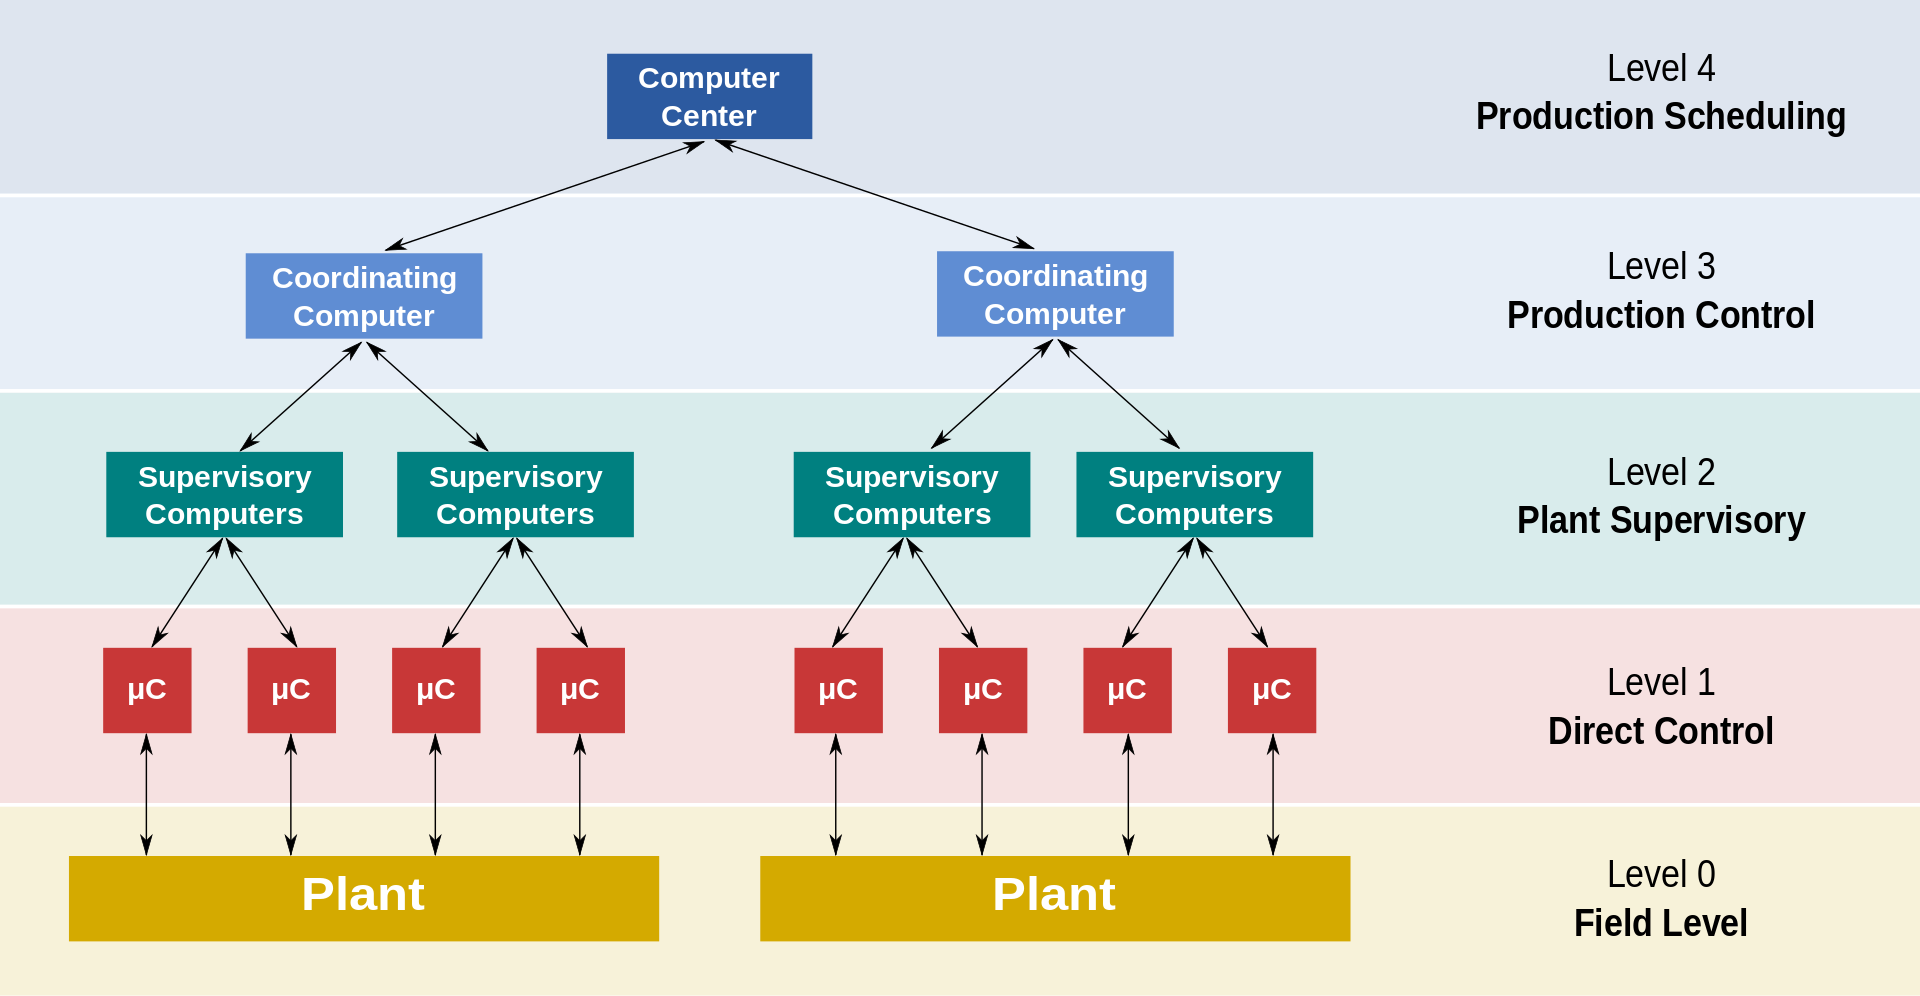
\includegraphics[scale=0.20]{layers_scada_architecture_wiki.png}
	\caption{SCADA architecture schema}
	\label{fig:SCADA_schema}
\end{figure}

SCADA architecture consists in \textbf{five layers} (Figure \ref{fig:SCADA_schema}):

\begin{itemize}
	\item Level 0 (\textbf{Field Level}): contains \textbf{field devices} (\ref{subsec:field_devs}), or \textit{sensors}.
	\item Level 1 (\textbf{Direct Control}): includes \textbf{local or remote controllers} such as \textbf{PLCs} (\ref{subsec:plc}) and \textbf{RTUs} (\ref{subsec:rtu}). Controllers interface directly to the field devices reading data from sensors and sending commands to actuators.
	\item Level 2 (\textbf{Plant Supervisory}): contains computer systems that \textbf{collate and store informations} from the previous level and provide a \textbf{Human-Machine Interface} (\textit{HMI}, \ref{subsec:hmi}) for operator control.
	\item Level 3 (\textbf{Production Control}): collect and aggregates data from the Plant Supervisory level to generate \textbf{reporting} to the Production Scheduling layer.
	\item Level 4 (\textbf{Production Scheduling}): includes business systems (such as ERP systems) used to \textbf{manage ongoing processes}.
\end{itemize}

Production Control level and Production Scheduling level are not directly connected to the process control, but concerned with monitoring production and targets and production scheduling level.

\subsection{Field devices}
\label{subsec:field_devs}
\textit{Field devices} are the \textbf{sensors} and \textbf{actuators} that are used to collect data from the process and control it. Examples of field devices include temperature sensors, pressure sensors, valves and pumps.

\subsection{IED} 
todo

\subsection{PLC}
\label{subsec:plc}
A \textit{Programmable Logic Controller} (PLC) is a \textbf{small and specialized industrial computer} having the capability of controlling complex industrial and manifacturing processes \cite{plc_definition}.

\bigskip
Compared to relay systems and personal computers, PLCs are optimized for control tasks and industrial environments: they are rugged and designed to withdraw harsh conditions such as dust, vibrations, humidity and temperature: they have more reliability than personal computers, which are more prone to crash, and they are more compact a require less maintenance than a relay system.
Furthermore, I/O interfaces are already on the controller, so PLCs are easier to expand with additional I/O modules (if in a rack format) to manage more inputs and ouputs, without reconfiguring hardware as in relay systems when a reconfiguration occours. 

\bigskip
PLCs are more \textit{user-friendly}: they are not intended (only) for computer programmers, but designed for engineers with a limited knowledge in programming languages: control program can be entered with a simple and intuitive language based on logic and switching operations instead of a general-purpose programming language (\textit{i.e.} C, C++, ...). 

\subsubsection{PLC Architecture}
The basic hardware architecture of a PLC consists of these elements \cite{plc_book}:

\begin{figure}[h]
	\centering
	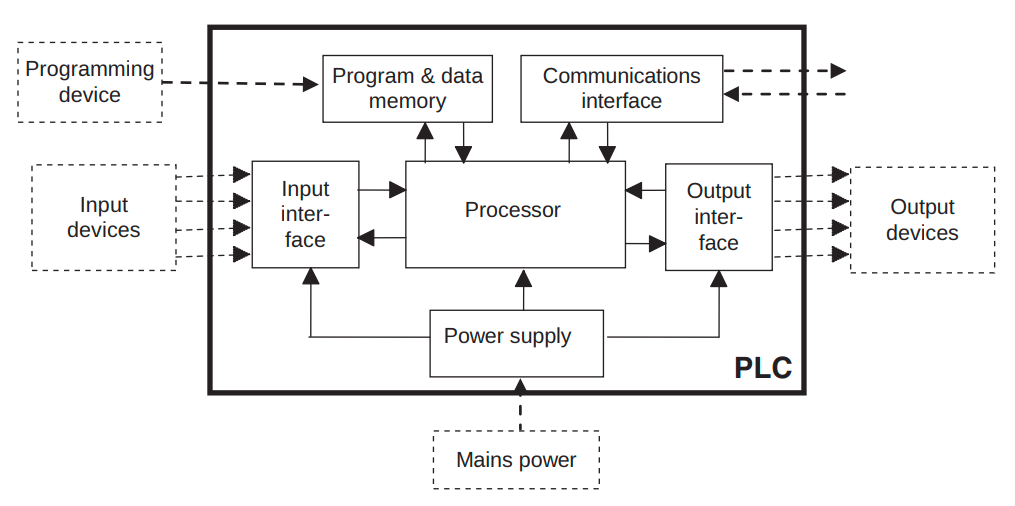
\includegraphics[scale=0.35]{plc_architecture.png}
	\caption{PLC architecture}
	\label{fig:PLC_architecture}
\end{figure}

\begin{itemize}
	\item \textbf{Processor unit (CPU)}: contains the microprocessor. This unit interpretes the input signals from I/O modules, executes the control program stored in the Memory Unit and sends the output signals to the I/O Modules.
	The processor unit also sends data to the Communication interface, for the communication with additional devices.
	\item \textbf{Power supply unit:} converts AC voltage to low DC voltage.
	\item \textbf{Programming device:} is used to store the required program into the memory unit.
	\item \textbf{Memory Unit:} consists in RAM memory and ROM memory. RAM memory is used for storing data from inputs, ROM memory for storing operating system, firmware and user program to be executed by the CPU.
	\item \textbf{I/O modules:} provide interface between sensors and final control elements (actuators).
	\item \textbf{Communications interface:} used to send and receive data on a network from/to other PLCs.
\end{itemize}

\begin{figure}[h]
	\centering
	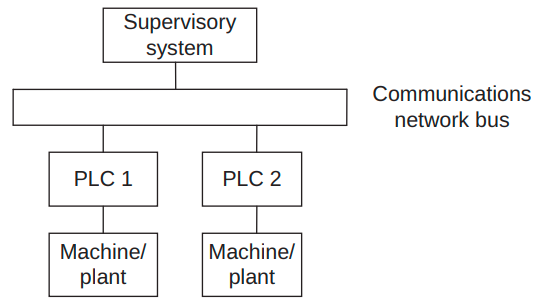
\includegraphics[scale=0.45]{plc_comm.png}
	\caption{PLC communication schema}
	\label{fig:PLC_comm}
\end{figure}

\subsubsection{PLC Programming}
\label{subsubsec:plc_programming}
Two different programs are executed in a PLC: the \textbf{operating system} and the \textbf{user program}.

\bigskip
The operating system tasks include executing the user program, managing memory areas and the \textit{process image table} (memory registers where inputs from sensors and outputs for actuators are stored).

\bigskip
The user program needs to be uploaded on the PLC via the programming device and runs on the process image table in \textit{scan cycles}: each scan is made up of three phases \cite{ceccato}:

\begin{enumerate}
	\item reading inputs from the process images table
	\item execution of the control code and computing the physical process evolution
	\item writing output to the process image table to have an effect on the physical process. At the end of the cycle, the process image table is refreshed by the CPU
\end{enumerate}

Standard PLCs \textbf{programming languages} are basically of two types: \textbf{textuals} and \textbf{graphicals}.
Textual languages include languages such as \textit{Instruction List} (IL) and \textit{Structured Text} (ST), while \textit{Ladder Diagrams} (LD), \textit{Function Block Diagram} (FBD) and \textit{Sequential Function Chart} (SFC) belong to the graphical languages.

\bigskip
Graphical languages are more simple and immediate comparing to the textual ones and are preferred by programmers because of their features and simplicity, in particular the \textbf{Ladder Logic programming} (see Figure \ref{fig:st_ll_comparison} for a comparison).

\begin{figure}[h]
	\centering
	\begin{subfigure}{0.47\textwidth}
		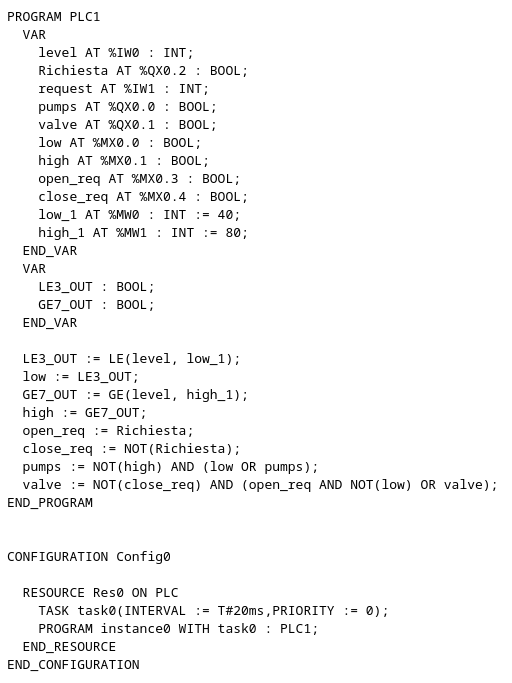
\includegraphics[scale=0.30]{st.png}
		\caption{Example of ST programming}
		\label{subfig:st_example}
	\end{subfigure}
	\hfill
	\begin{subfigure}{0.47\textwidth}
		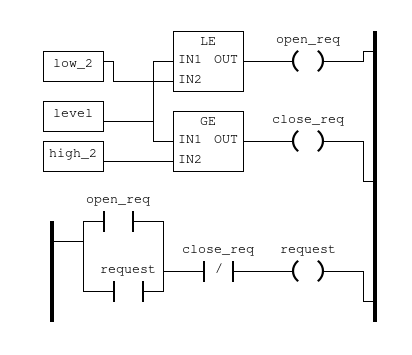
\includegraphics[scale=0.55]{ll.png}
		\caption{Example of Ladder Logic}
		\label{subfig:ladder_logic_example}
	\end{subfigure}
	\caption{Comparison between ST language and Ladder Logic}
	\label{fig:st_ll_comparison}
	
\end{figure}

\subsubsection{PLC Security}
\label{subsubsec:plc_security}
PLCs were originally designed to operate as closed systems, not connected and exposed to the outside world via communication networks: the question of the safety of these systems, therefore, was not a primary aspect. The advent of the Internet has brought undoubted advantages, but has introduced problems relating to the safety and protection of PLCs from external attacks and vulnerabilities.

\subsection{RTU}
\label{subsec:rtu}
\textit{Remote Terminal Units} (RTUs) are computers with radio interfacing similar to PLCs: they transmit telemetry data to the control center or the PLCs
and use messages from the master supervisory system to control connected objects \cite{rtu_definition}.

\bigskip
RTUs are intended to work in remote areas communicating via wireless connections, while PLCs are meant to work locally with a high speed wired connection; due to this reason, RTUs can operate in low power modes for long periods of time using solar panels or batteries, with less energy consumption than PLCs.

\bigskip
Industries that use RTUs include telecom, rail, utilities.

\subsection{HMI}
\label{subsec:hmi}
The Human-Machine Interface (HMI) is the interface that operators use to interact with the ICS. HMIs can be used to display process data, make control decisions, and configure the ICS.

\subsection{Cybersecurity components}
Cybersecurity components: This can include firewalls, intrusion detection and prevention systems (IDPS), and security information and event management (SIEM) systems. These are used to protect the ICS from cyber threats and vulnerabilities.

\subsection{Communication Networks}
Communication Networks are the networks that are used to connect the different components of the ICS and allow them to communicate with each other. Communication networks can include wired and wireless networks, such as Ethernet, MODBUS, and DNP3.

\section{ICS Communication Protocols}
\label{sec:ics_protocols}

\subsection{Modbus}

\subsection{Ethernet/IP}

\subsection{Other Protocols}

\vfill
%
%Test cite \cite{ceccato} \\
%test cite 2 \cite{itrust_swat} \\
%test cite 3 \cite{itrust_site} \\
%test cite 3 \cite{itrust_invariants_paper}\\
%
%\begin{figure}[h]
%	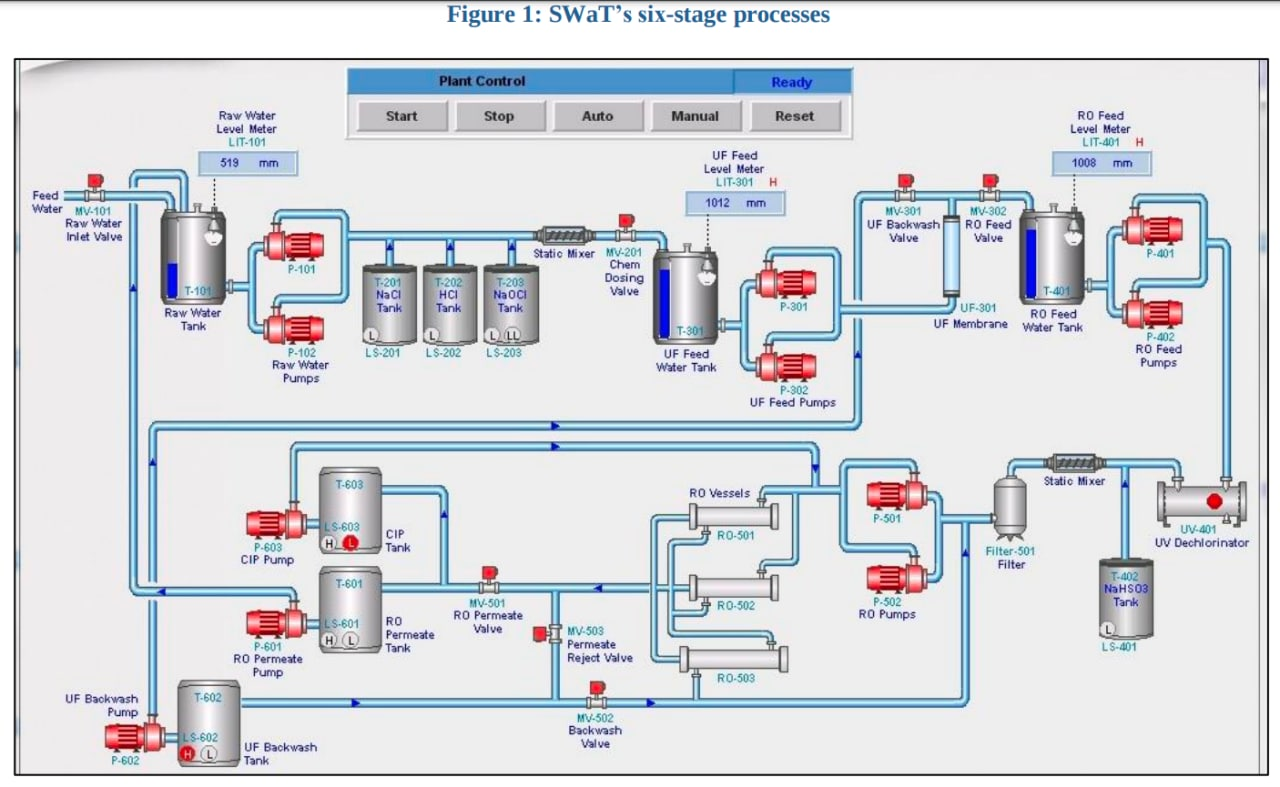
\includegraphics[scale=0.3]{swat_schema_2}
%	\caption{SWaT schema}
%	\label{fig:Schema SWaT}
%\end{figure}
%
%\begin{table}
%	\centering
%	\begin{tabular}{||c c c c||} 
%		\hline
%		Col1 & Col2 & Col2 & Col3 \\ [0.5ex] 
%		\hline
%		 & & & \\
%		1 & 6 & 87837 & 787 \\ 
%		2 & 7 & 78 & 5415 \\
%		3 & 545 & 778 & 7507 \\
%		4 & 545 & 18744 & 7560 \\
%		5 & 88 & 788 & 6344 \\ [1ex] 
%	\end{tabular}
%	\label{table:1}
%\end{table}
